\chapter{Decripción del código} \label{chap:descripcion_codigo}
\section{Clase Main.} \label{sec:main}
\section{Variables de iniciación} \label{subsec:variables}
las variables que se usaron, son las variables que definen la lógica del programa.

\begin{figure}[H]
\centering
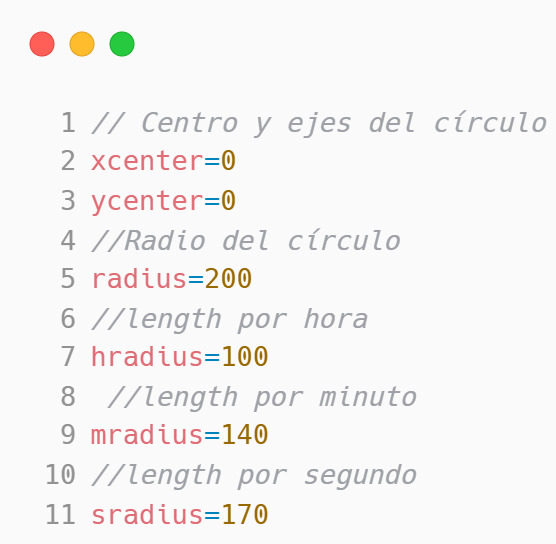
\includegraphics[width=0.4\textwidth]{../img/chapter02/2.png}
\caption{Varibles inicializadas}
\label{fig:variables_iniciales}
\end{figure}

Como se observa en la figura \ref{fig:variables_iniciales}, están los ejes \textbf{x} y \textbf{y}, Tenemos los radios del círculo para éste caso, los cuales están los respectivos radios para las manecillas del reloj (segundo definido con valor 200, minuto 100 y hora 170).

\subsection{Clase Clock.} \label{subsec:clock}
Como se explicón en el apartado \ref{subsec:arbol}, conversamos de una clase que tiene que los métodos que trabajan con las animaciones que simula un reloj andando (que no es algo obligatorio para el laboratorio, es un extra que trae el proyecto que edité).

\begin{figure}[H]
	\centering
	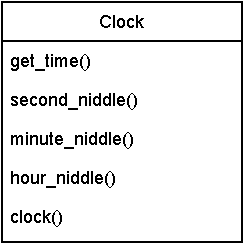
\includegraphics[width=0.4\textwidth]{../img/chapter02/4.pdf}
	\caption{Clase Clock}
	\label{fig:clock}
\end{figure}

Ésta clase, como se muestra en la figura \ref{fig:clock}, tiene los métodos \textbf{get\_time, second\_niddle, minute\_niddle, hour\_niddle y clock}.

\subsection{Clase Display.} \label{subsec:display}
Ésta clase sólo tiene un método que es, irónicamente, un método que tiene el mismo nombre que la clase

\begin{figure}[H]
	\centering
	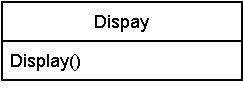
\includegraphics[width=0.4\textwidth]{../img/chapter02/5.pdf}
	\caption{Clase Clock}
	\label{fig:clock}
\end{figure}

La función de la ésta clase, maneja la posición, el tamaño, y demás items de las ventanas visuales del programa.

\subsection{Clase Draw.} \label{subsec:draw}

Ésta clase contiene los métodos lineDDA, draw\_circle, draw, setPixel y glutPrint.

\begin{figure}[H]
	\centering
	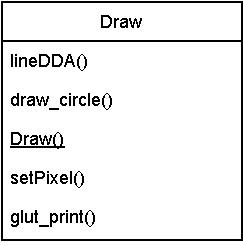
\includegraphics[width=0.2\textwidth]{../img/chapter02/6.pdf}
	\caption{Clase Clock}
	\label{fig:clock}
\end{figure}





